%   DOCUMENT CLASS  %%%%%%%%%%%%%%%%%%%%%%%%%%%%%%%%%%%%%%%%%%%%%%%%%%%%%%%%%%%
%
%   Use the `sfuthesis` class to format your thesis. If your program does not
%   require a thesis defence, use the class option `undefended` like so:
%
%     \documentclass[undefended]{sfuthesis}
%
%   To generate a signature page for your defence, use the `sfuapproval` class
%   instead, by replacing the below line with
%
%     \documentclass{sfuapproval}
%
%   For more information about thesis formatting requirements, go to
%
%     http://www.lib.sfu.ca/help/publish/thesis
%
%   or ask a thesis advisor at the SFU Research Commons.
%

\documentclass{sfuthesis}



%   DOCUMENT METADATA  %%%%%%%%%%%%%%%%%%%%%%%%%%%%%%%%%%%%%%%%%%%%%%%%%%%%%%%%
%
%   Fill in the following information for the title page and approval page.
%

\title{Temporal Consistency in Learning Action Values for Volleyball}
\thesistype{Project}
\author{Martin Ambrozic}
\previousdegrees{%
	M.Sc., Delft Technical University, 2013\\
	B.Sc., University of Ljubljana, 2011}
\degree{Master of Science}
\discipline{Computing Science}
\department{Department of Computing Science}
\faculty{Faculty of Applied Science}
\copyrightyear{2021}
\semester{Spring 2021}
\date{January 26, 2021}

\keywords{Action Values, Volleyball, Reinforcement Learning, Machine Learning}

\committee{%
	\chair{Ghassan Hamarneh}{Professor\\School of Computing Science}
	\member{Oliver Schulte}{Senior Supervisor\\Professor\\School of Computing Science}
	\member{Mo Chen}{Internal Examiner\\Assistant Professor\\School of Computing Science}
	\member{Steven Ruuth}{External Examiner\\Professor\\Department of Mathematics}
}



%   PACKAGES %%%%%%%%%%%%%%%%%%%%%%%%%%%%%%%%%%%%%%%%%%%%%%%%%%%%%%%%%%%%%%%%%%
%
%   Add any packages you need for your thesis here.
%   You don't need to call the following packages, which are already called in
%   the sfuthesis class file:
%
%   - appendix
%   - etoolbox
%   - fontenc
%   - geometry
%   - lmodern
%   - nowidow
%   - setspace
%   - tocloft
%
%   If you call one of the above packages (or one of their dependencies) with
%   options, you may get a "Option clash" LaTeX error. If you get this error,
%   you can fix it by removing your copy of \usepackage and passing the options
%   you need by adding
%
%       \PassOptionsToPackage{<options>}{<package>}
%
%   before \documentclass{sfuthesis}.
%
%   The following packages are a few suggestions you might find useful.
%
%   (1) amsmath and amssymb are essential if you have math in your thesis;
%       they provide useful commands like ``blackboard bold'' symbols and
%       environments for aligning equations.
%   (2) amsthm includes allows you to easily change the style and numbering of
%       theorems. It also provides an environment for proofs.
%   (3) graphicx allows you to add images with \includegraphics{filename}.
%   (4) hyperref turns your citations and cross-references into clickable
%       links, and adds metadata to the compiled PDF.
%   (5) pdfpages lets you import pages of external PDFs using the command
%       \includepdf{filename}. You will need to do this if your research
%       requires an Ethics Statement.
%

\usepackage{amsmath}                            % (1)
\usepackage{amssymb}                            % (1)
\usepackage{amsthm}                             % (2)
\usepackage{graphicx}                           % (3)
\usepackage{multirow}
\usepackage{makecell}
\usepackage[pdfborder={0 0 0}]{hyperref}        % (4)
% \usepackage{pdfpages}                         % (5)
% ...
% ...
% ...
% ... add your own packages here!




%   OTHER CUSTOMIZATIONS %%%%%%%%%%%%%%%%%%%%%%%%%%%%%%%%%%%%%%%%%%%%%%%%%%%%%%
%
%   Add any packages you need for your thesis here. We've started you off with
%   a few suggestions.
%
%   (1) Use a single word space between sentences. If you disable this, you
%       will have to manually control spacing around abbreviations.
%   (2) Correct the capitalization of "Chapter" and "Section" if you use the
%       \autoref macro from the `hyperref` package.
%   (3) The LaTeX thesis template defaults to one-and-a-half line spacing. If
%       your supervisor prefers double-spacing, you can redefine the
%       \defaultspacing command.
%

\frenchspacing                                    % (1)
\renewcommand*{\chapterautorefname}{Chapter}      % (2)
\renewcommand*{\sectionautorefname}{Section}      % (2)
\renewcommand*{\subsectionautorefname}{Section}   % (2)
% \renewcommand{\defaultspacing}{\doublespacing}  % (3)
% ...
% ...
% ...
% ... add your own customizations here!




%   FRONTMATTER  %%%%%%%%%%%%%%%%%%%%%%%%%%%%%%%%%%%%%%%%%%%%%%%%%%%%%%%%%%%%%%
%
%   Title page, committee page, copyright declaration, abstract,
%   dedication, acknowledgements, table of contents, etc.
%
%   If your research requires an Ethics Statement, download one from the
%   SFU library website and uncomment the appropriate lines below.
%

\begin{document}
	
	\frontmatter
	\maketitle{}
	\makecommittee{}
	
	\begin{abstract}
		Learning the value of actions taken during a match is a key idea in sports analytics with applications such as player ranking, tactical insight and outcome prediction. We compare two fundamentally different approaches for learning action values on a novel play-by-play volleyball dataset. In the first approach, we employ regression models that implicitly assume statistical independence of data samples. In the second approach, we use a deep reinforcement learning model, explicitly enforcing the sequential nature of the data in the learning process. We find that temporally independent regression can in certain settings outperform the reinforcement learning approach in terms of predictive accuracy, but the latter performs much better when temporal consistency is required. We also consider a mimic regression tree as a way to add interpretability to the deep reinforcement learning approach. Finally, we examine the computed action values and perform a number of example analyses to verify their validity.
	\end{abstract}
	
	
	\begin{dedication}
		To Patrick, for being my anchor through 2020.
	\end{dedication}
	
	
	\begin{acknowledgements}
		I would like to extend my deepest thanks to my supervisor Oliver Schulte for his unwavering guidance and support throughout my studies in Computing Science and for his help in the creation of this project.
	\end{acknowledgements}
	
	\addtoToC{Table of Contents}%
	\tableofcontents%
	\clearpage
	
	\addtoToC{List of Tables}%
	\listoftables%
	\clearpage
	
	\addtoToC{List of Figures}%
	\listoffigures%
	\clearpage
	
	
	
	
	
	%   MAIN MATTER  %%%%%%%%%%%%%%%%%%%%%%%%%%%%%%%%%%%%%%%%%%%%%%%%%%%%%%%%%%%%%%
	%
	%   Start writing your thesis --- or start \include ing chapters --- here.
	%
	
	\mainmatter%
	
	%\chapter{Introduction}
	
	%By default, only works cited in the text will be added to the bibliography~\cite{latexcompanion}.
	\chapter{Introduction}
	
	Increasing volume of collected data in all kinds of sports has made machine learning techniques a quickly developing area in sports science, but progress varies depending on the particular sport in question \cite{claudino2019current}. Learning the value of actions taken during a match is key to sports analytics. It offers applications such as player evaluation (by aggregating a player's action values) strategic analysis (by comparing actions in a given context) or even match outcome prediction \cite{albert2017handbook, liu2018deep, pappalardo2018quantifying, pettigrew2015assessing, schulte2017markov}.
	
	An action value function maps the match state and an action to a real value, which measures the team's chance of success after the action is taken. Two fundamental approaches have been explored for learning action values:
	\begin{enumerate}
		\item A regression approach where state-action inputs are treated as the independent variable and success chance as the dependent target variable. The regression approach implicitly assumes that the values for different state-action pairs are statistically independent of each other. However, in the actual data, the chances of success for successive state-action pairs are highly correlated. Examples of this approach include work on soccer data in \cite{decroos2019actions} and \cite{pappalardo2019playerank}.
		\item Temporal difference learning, which exploits this correlation by forcing success predictions for successive state-action pairs to be consistent with each other, such as in \cite{liu2018deep} and \cite{schulte2017markov}.
	\end{enumerate}
	This project compares the two approaches on a novel volleyball dataset collected in the past three seasons through a collaboration with the University of British Columbia Men's Volleyball program.
	
	\section{Preliminaries and Objectives}
	\subsection{Markov Decision Process}
	A Markov decision process (abbreviated as MDP) is a discrete-time stochastic process consisting of a set of states $S$, a set of actions $A$, and a transition function $P_a(s,s')$ which gives the transition probability from state $s$ into state $s'$ given that action $a$ was taken. 
	\subsection{Action Value Function}
	\label{section:value-function}
	If a reward function $R_a(s,s')$ is provided along with an MDP, this allows for evaluation of actions taken in terms of expected future reward. The Q function, given for an action taking policy $\pi$ as:
	\begin{equation}
		Q_\pi(s,a) = \mathbb{E} \left[  R_{t+1} + \gamma Q_{\pi}(S_{t+1}, A_{t+1}) \, | \, S_t = s, A_t = a \right]
	\end{equation}
	formalizes this. Here $R_{t+1}$ is shorthand for $R_a(S_t,S_{t+1})$, i.e. the reward obtained by taking action $a$ in state $S_t$ and proceeding to state $S_{t+1}$. A discounting factor $\gamma$ is used to avoid infinitely large accumulation of rewards in some applications, but following the example in hockey-related work \cite{liu2018deep, schulte2017apples, schulte2017markov}, we set $\gamma=1$ in our experiments. The main motivation is that in volleyball, points scored are worth the same regardless of when they are scored and longer rallies do not diminish the reward at the end.
	\subsection{Objectives}
	The aim of this project is to:
	\begin{enumerate}
		\item Construct an MDP from volleyball play-by-play event data. The states of the MDP represent match context and the actions correspond to player actions on the court.
		\item Compute an action value function using:
		\begin{enumerate}
			\item regression learning that assumes temporal independence,
			\item reinforcement learning that enforces temporal consistency
		\end{enumerate}
		and compare results.
	\end{enumerate}  
	
	\section{Related Work}
	\subsection{Computing Action Values}
	The concept of an action value function has been applied to event data in a number of different sports. In \cite{cervone2014pointwise}, expected value of possessions in basketball (equivalent to a Q function) was used on an NBA dataset. Similarly, soccer actions were evaluated in terms of scoring probability in \cite{decroos2019actions}. However, this project relies mostly on work in the hockey context done by Liu, Routley and Schulte \cite{liu2018deep, routley2015markov, schulte2017markov, schulte2017apples} on large NHL event datasets. Their work has further been extended to consider pairs of players appearing on the ice together in \cite{Ljung2019}. A similar action value based approach was also taken in \cite{kaplan2014markov}.
	\subsection{Volleyball Statistical Analysis}
	In volleyball, there have been previous applications of statistical methods involving Markov chains, but the dataset concerned actions of only one of the two teams and no game context such as current score was included. This is in contrast to our dataset, where both opponents' data is included. Skill importance was computed in this fashion in \cite{miskin2010skill}, rally winning probabilities were computed in \cite{florence2008skill} and home advantage was brought into question in \cite{alexandros2012existence}.
	\subsection{Machine Learning in Volleyball}
	Moving to more recent research than the purely statistical research listed in the previous section, machine learning has been applied to volleyball data with the goal of predicting future team rankings from win/loss data in \cite{tumer2017prediction}.  Deep models were employed for activity recognition on video in \cite{ibrahim2018deep} and \cite{kautz2017activity}, with the objective of determining training load and injury risk. In \cite{wenninger2020performance} and \cite{van2016analyzing}, analysis and prediction of attack patterns was carried out using artificial intelligence methods and \cite{wang2018volleyball} tackled classification of players into skill levels based on motion data from wearable devices.
	
	Despite progress of machine learning in a variety of fields in volleyball, however, we did not encounter a context-aware approach to estimating action values  that this project applies to a volleyball event dataset.
	
	\section{Report Structure}
	This report is structured as follows:
	\begin{itemize}
		\item In Chapter 2, we describe the volleyball dataset used and discuss the modelling decisions made in the process of constructing our MDP.
		\item Chapter 3 gives details on the various machine learning models used in computing the action value function.
		\item In Chapter 4, we discuss comparison metrics between the models and give results.
		\item Chapter 5 gives some examples of potential applications of the action value function in a practical setting.
		\item Chapter 6 draws conclusions and suggests future work.
	\end{itemize}
	
	\chapter{Dataset and the Markov Decision Process}
	
	\section{Dataset Description}
	The volleyball dataset was collected in collaboration with the University of British Columbia's men's volleyball programme. The UBC Thunderbirds compete in the Canada West division of U-Sports volleyball, which is the highest level of volleyball university competition in Canada. Their regular season consists of a double round robin phase, where they play each of the other Canada West teams twice, and a play-off phase, where top seeded teams play a single elimination bracket to determine the conference champion as well as participants in the U-Sports national final tournament. During the data collection time window, 12 teams participated in the Canada West competition, except in 2017/2018, where 13 teams competed.
	
	The collection process was manual, using specialized software to record play-by-play data, either live at the game or after the fact using game video. In the former case, a second pass was needed to ensure quality and completeness of data. The format used was introduced by the company Data Project based in Salerno, Italy and has become widely adopted in professional and international volleyball. Both teams' actions were included for every game.
	
	The dataset contains data from all games played by UBC over three seasons. Additionally, a number of matches between other teams in Canada West were included, originally intended for the purpose of tactical preparation for an upcoming opponent.
	
	Table \ref{tab:data-numbers} describes the dataset size in terms of games, sets, rallies and game events.\\
	\begin{table}[ht]
		\centering
		\begin{tabular}{c|c|c|c|c}
			& \textbf{Games} & \textbf{Sets} & \textbf{Rallies} & \textbf{Events} \\ \hline
			\textbf{Contained in Data} & 204            & 764           & 34,242           & 146,050        
		\end{tabular}
		\caption{Dataset size description in various terms.}
		\label{tab:data-numbers}
	\end{table}
	\\Each entry in the dataset corresponds to an action event by a player in the game. We differentiate 7 action types:
	\begin{itemize}
		\item \textbf{Serve}: first contact of the serving team, the action of putting the ball into play over the net from behind the baseline.
		\item \textbf{Receive}: first contact of the team receiving the opponent's serve.
		\item \textbf{Set}: Second contact on either side, the aim of which is to deliver the ball to an attacker.
		\item \textbf{Attack}: Usually the third contact of either team, spiking the ball over the net with the aim of scoring by hitting the ground in the opponent's court.
		\item \textbf{Block}: The action of one or more players by the net attempting to defending against an attack by deflecting the ball back to the opponent's court as it crosses the net.
		\item \textbf{Dig}: The defensive action against an opponent's attack, volleying the ball before it contacts the ground.
		\item \textbf{Free-ball}: The first contact of a team after the opposing team failed to produce a proper attack and volleyed an 'easy ball' over the net.
	\end{itemize}
	Further, the outcome of each action is recorded, ranging from '=' (double negative), through '-' (negative), '/', '!', '+' (positive) and '\#' (double positive). The meanings of these symbols vary by action type, but in general double negative corresponds to an error (awarding the rally to the opponent) and double positive is a winning or perfect outcome, eg. a scoring attack.
	
	For most actions, the execution location is also recorded, as well as the trajectory location for attack and serve actions. Finally, we also record the context, i.e. the state of the game, including the current set number (1 through maximum 5) and the points scored by each team in the current set (usually between 0 and 25, but can be higher in a 'win by 2' scenario). Table \ref{tab:data-fields} summarizes the context and action-related fields recorded in the dataset.
	\begin{table}[ht]
		\centering
		\begin{tabular}{c|c|c|c|c}
			\textbf{Action Field} & \textbf{Player, Team} & \textbf{Type} & \textbf{Outcome} & \textbf{Location, Trajectory}         \\ \hline
			\textbf{Range} & categorical           & 7 categories  & 6 categories     & \makecell[c]{Discretized\\ 12-by-6 grid of locations}
		\end{tabular}
		\\ \vspace{0.75cm}
		\begin{tabular}{c|c|c}
			\textbf{Context Field} & \textbf{Set Number} & \textbf{Set Scores}    \\ \hline
			\textbf{Range} & Integers 1-5        & Integers 0-31
		\end{tabular}
		\caption{Summary of fields in the volleyball dataset. Action-related fields on top, context-related fields on the bottom.}
		\label{tab:data-fields}
	\end{table}
	
	\section{The Markov Decision Process}
	\label{section-mdp}
	
	In volleyball, a rally is a sequence of actions beginning with the serve and ending with one of the teams scoring a point. We model every rally as a sequence of states and actions of a Markov Decision Process (abbreviated as MDP). We incorporate context and history in the state space similar to \cite{schulte2017markov}.
	
	In determining the extent of action history to include, we consider the distribution of rally lengths (in terms of the number of actions). Figure \ref{fig:rally-lengths} shows a histogram of rally lengths found in the dataset. We adopt a maximum history window of 9 actions, which means 96\% of all rallies are encompassed in full from their beginning.\\
	\begin{figure}
		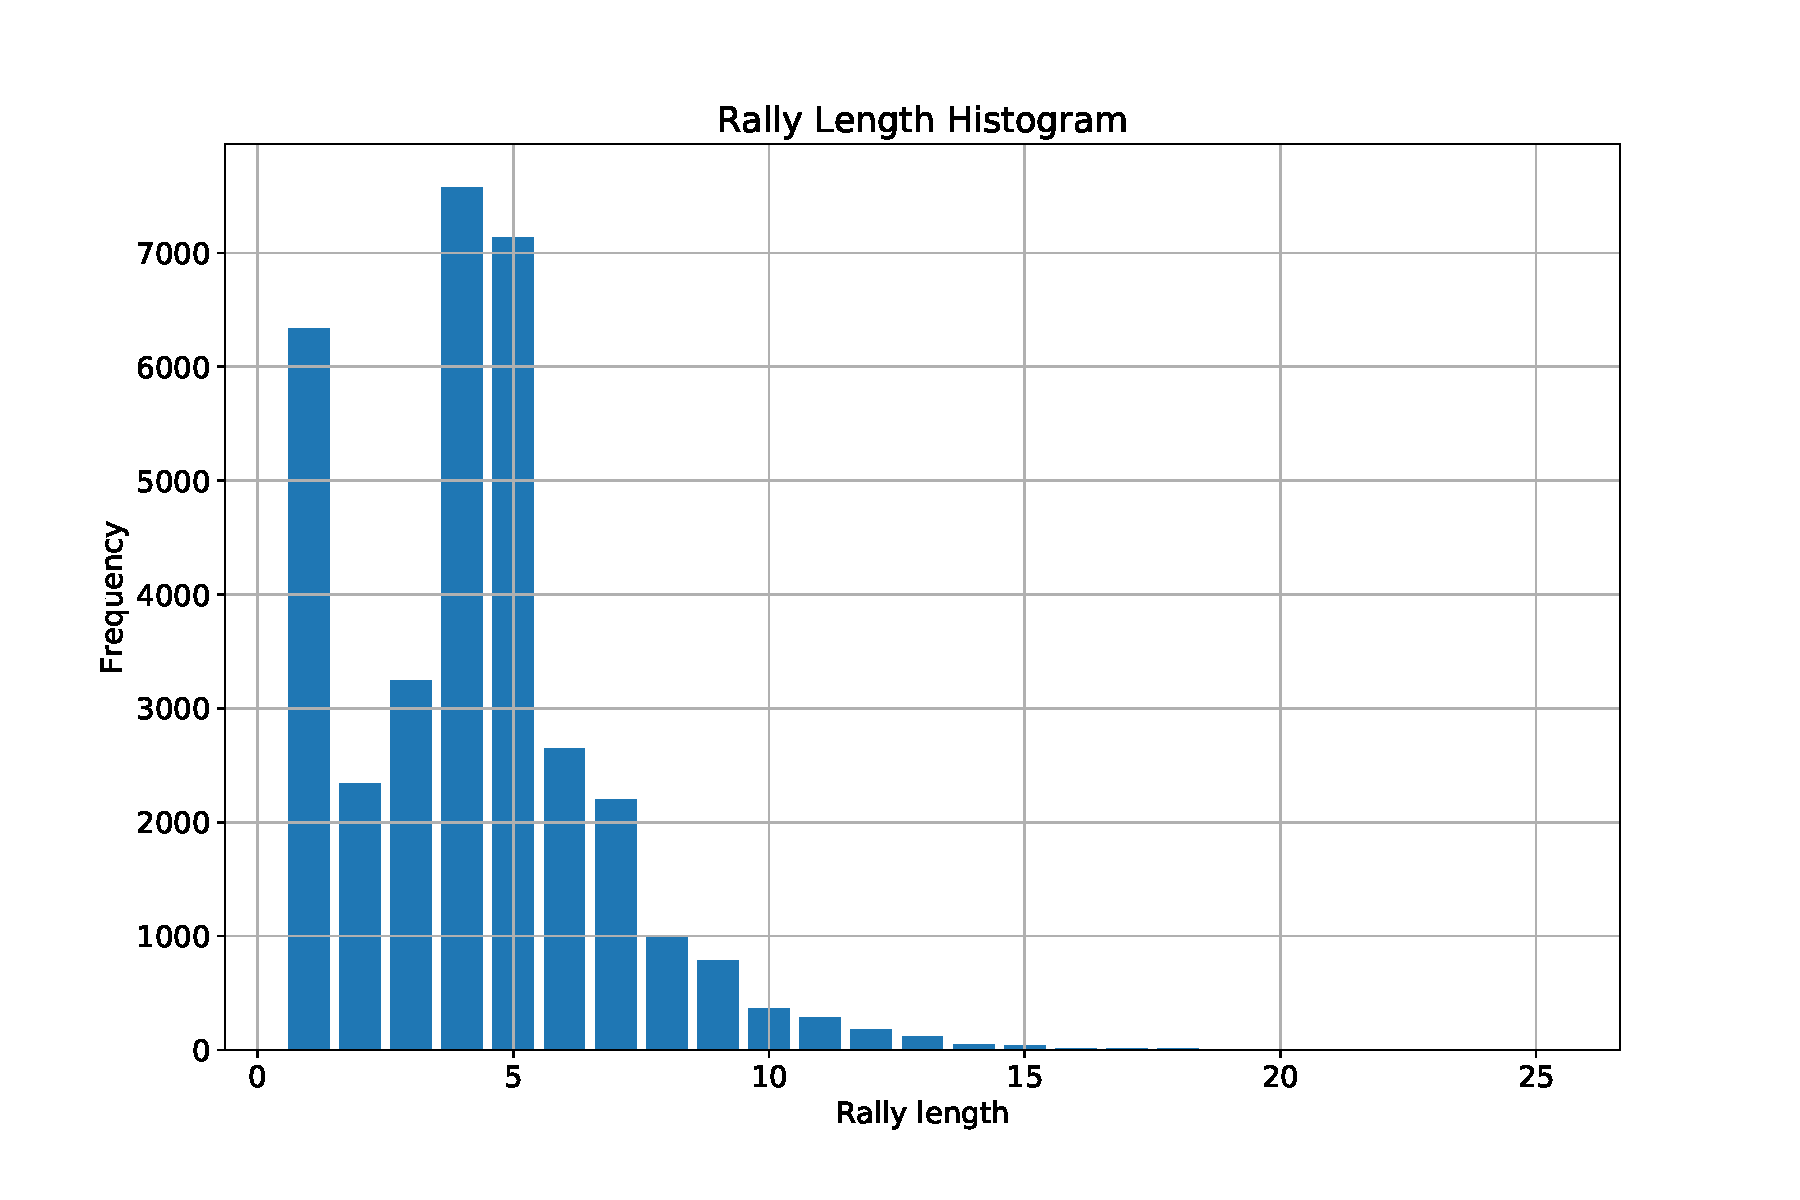
\includegraphics[scale=0.5]{img/rally_lengths.pdf}
		\caption{Rally length histogram for the volleyball dataset.}
		\label{fig:rally-lengths}
	\end{figure}
	\\
	Every rally corresponds to a walk through the states of the MDP, where the action taken by either team determines the next state. Eventually one of the teams wins the point and the walk terminates. We model this by a reward function $r: S \times A \rightarrow \mathbb{Z}$, where $S$ is the state space, $A$ is the action space and
	\begin{equation}
		r(s,a) =
		\begin{cases} 
			1 & \text{if home team wins the rally} \\
			-1 & \text{if away team wins the rally} \\
			0 & \text{otherwise.} 
		\end{cases}
		\label{eq:reward_function}
	\end{equation}
	We denote the reward value at step $t$ of the walk as $r_t$. In this setting, our quantity of interest is the state-action value function, also commonly called the Q function \cite{sutton2018reinforcement}. It expresses the expected future reward given the current state and action at step $k$, assuming future actions follow policy $\pi$:
	\begin{equation}
		Q_\pi(s,a) = \mathbb{E} \left[ \sum_{t \ge k} \gamma^{t-k} r_{t} \ | \ s_k = s, a_k = a \right]\\
		\label{eq:qfunction}
	\end{equation}
	Often in reinforcement learning applications, the objective is to compute the optimal policy $\pi^*$. This is {\em not} the case in this context, as the objective is only to {\em evaluate} the match states and actions {\em given} the policy observed in the data. The observed policy represents the behaviour of the average volleyball player. We thus omit the subscript $\pi$ from here on. Additionally, as discussed in section \ref{section:value-function}, we use a discounting factor of $\gamma=1$ for all derivations and experiments to follow.
	
	
	\chapter{Models}
	
	\section{Temporally Independent Models}
	
	We first consider regression models that treat data samples as independent. The Q function gives the expected future reward in an episode starting from a given state-action pair by equation \eqref{eq:qfunction}. Treating the current state and action as the independent variable $x$ and the expected reward as the output, we can formulate this as a regression problem, where the target value $R(s,a)$ for each sample in the training data is $1$ or $-1$, depending on which team eventually won the rally. If we train a function estimator $Q'$ that minimizes the mean squared error
	\begin{equation}
		\frac{1}{|X|}\sum_{x \in X} (Q'(x) - R(x))^2,
		\label{eq:mse}
	\end{equation}
	then $Q'(s,a)$ will approximate the conditional expected value
	$$\mathbb{E} \left[R \, | \, x \right].$$
	This follows from the property that conditional expectation of the target in general minimizes mean squared error. See, e.g. Bishop \cite{bishop2006pattern} section 1.5.5 for a derivation of this property. In other words, since $x$ is a state-action pair sample and $R(x)$ is the eventual reward, $Q'(x)$ will approximate the Q function. We now consider specific models that follow this approach.
	
	\subsection{Decision Tree}
	
	Decision trees are an appealing model because they offer interpretable function approximation modelled as a sequence of simple decisions. We used a regression tree class from the Python scikit-learn package. Due to categorical fields in the dataset, a pre-processing step was needed, encoding the categorical data using a number of binary 'dummy' columns.
	
	To avoid overfitting, the maximum depth of the tree was limited and 5-fold cross-validation was used to determine the best value for maximum depth (i.e. the one that gave the minimal mean squared error averaged over the 5 cross-validation runs). 
	
	Table \ref{tab:tree-mse} shows experiment results for a range of maximal depth values. Setting the depth limit to 10 was adopted as the best model based on the mean squared error values shown.\\
	\begin{table}[ht]
		\centering
		\begin{tabular}{c|cccccc}
			\textbf{max\_depth}                & 8      & 9      & 10     & 11     & 12     & 13     \\ \hline
			\textbf{mean cross-validation MSE} & 0.6476 & 0.6302 & 0.6248 & 0.6260 & 0.6335 & 0.6448
		\end{tabular}
		\caption{Mean MSE values for 5-fold cross-validation using a regression tree model with varying maximal depth.}
		\label{tab:tree-mse}
	\end{table}
	\\A distinct feature of tree models is the ability to plot and examine the tree structure. We show the first three levels of the adopted tree in Figure \ref{fig:tree-plot}. We notice the top level splits mostly concern the most recent two action outcomes, which seems sensible. Interestingly, it looks like action outcomes are considered before action types. This is likely due to the fact that outcome symbols, especially the extremes '\#' and '=', share the meaning of 'point scored' and 'point lost' across several volleyball skills.
	\begin{figure}[ht]
		\hspace{-3cm}
		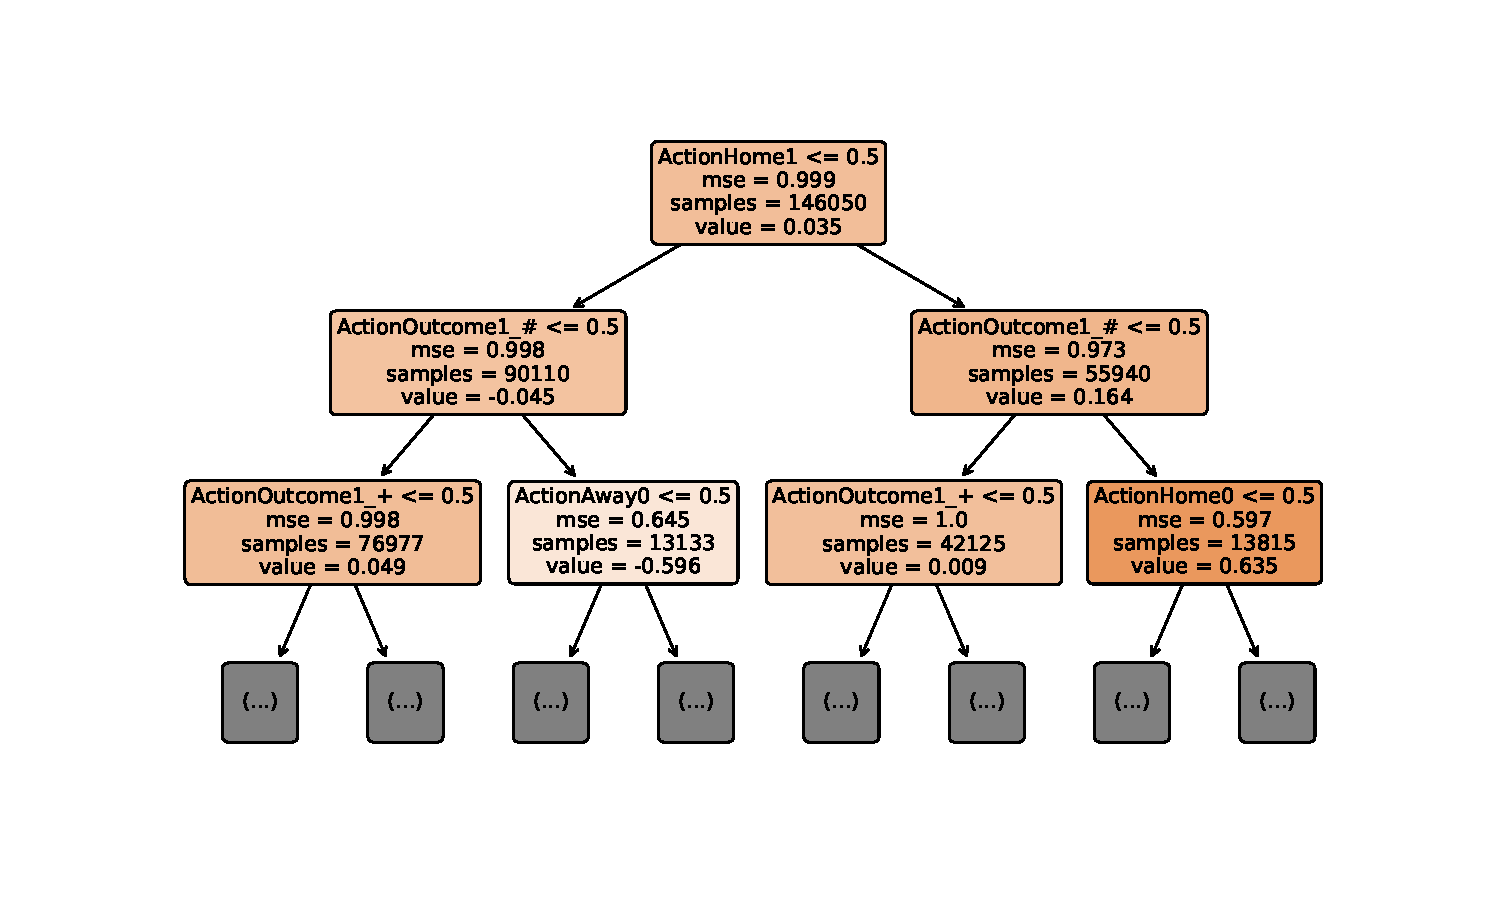
\includegraphics[scale=0.48]{img/tree_plot.pdf}
		\caption{First levels of the regression tree structure.}
		\label{fig:tree-plot}
	\end{figure}
	
	\subsection{Random Forest}
	
	While decision trees are an appealing model in terms of simplicity and interpretability, we wish to examine a potentially stronger regression model by using ensemble methods. The random forest model from the Python scikit-learn package allows for a straightforward implementation of an ensemble of trees. We use the same pre-processing steps as above and train an ensemble of 10 decision tree estimators (experiments showed that using more estimators beyond 10 did not provide a significant decrease in mean squared error). Table \ref{tab:forest-mse} shows mean MSE values for 5-fold cross-validation using a random forest model. An improvement over using a single decision tree can clearly be observed.\\
	\begin{table}[ht]
		\centering
		\begin{tabular}{c|ccccc}
			\textbf{max\_depth}                & 10      & 11      & 12     & 13     & 14       \\ \hline
			\textbf{mean cross-validation MSE} & 0.6177 & 0.6159 & 0.6170 & 0.6192 & 0.6222
		\end{tabular}
		\caption{Mean MSE values for 5-fold cross-validation using a regression random forest model with varying maximal depth.}
		\label{tab:forest-mse}
	\end{table}
	
	\subsection{Regression Neural Network}
	
	We also explore the option of a neural network as a regression model. After experimenting with a range of hidden layers, activation functions and node counts, we decide on the following architecture:
	\begin{itemize}
		\item First dense layer of 200 nodes with RelU activation,
		\item Second dense layer of 20 nodes with RelU activation,
		\item Output layer with $\tanh$ activation.
	\end{itemize}
	The final activation is a $\tanh$ function because we desire an output range of $[-1,1]$ to match the action value function. Similarly to previous models, we employ 5-fold cross validation to determine the best number of training epochs to prevent overfitting to the training data. Table \ref{tab:nn-mse} shows mean MSE values for a range of training epoch counts. We adopted 7 epochs as the best value in further experiments.
	\begin{table}[ht]
		\centering
		\begin{tabular}{c|ccccccc}
			\textbf{epochs} & 4 & 5 & 6 & 7 & 8 & 9 & 10 \\ \hline
			\textbf{mean cross-val. MSE} & 0.6162 & 0.6145 & 0.6139 & 0.6116 & 0.6147 & 0.6142 & 0.6154
		\end{tabular}
		\caption{Mean MSE values for 5-fold cross-validation using a regression neural network model with varying number of training epochs.}
		\label{tab:nn-mse}
	\end{table}
	
	\section{Temporally Consistent Models}
	
	In this section we consider a reinforcement learning approach, where the underlying MDP is exploited and the sequential nature of the data is explicitly used in the learning process. More specifically, the state-action value function has the recurrent property:
	\begin{equation}
		Q(s,a) = r(s,a) +\sum_{s',a' \in S \times A} T(s,a,s',a') \; Q(s', a')
		\label{eq:q-recursive}
	\end{equation}
	where $T(s,a)$ denotes the probability that the state-action pair $(s',a')$ follows $(s,a)$ in the MDP. Equation \eqref{eq:q-recursive} includes assumptions made in section \ref{section-mdp}.
	
	\subsection{Neural Network}
	
	We base our neural network architecture on the approach in \cite{liu2018deep} that proved successful for deep learning using NHL hockey data. After some experiments with the number of nodes, we adopt the following structure for our reinforcement learning based neural network:
	\begin{itemize}
		\item First layer containing 256 LSTM nodes for sequence processing,
		\item Hidden dense layer of 1000 nodes with RelU activation,
		\item Output layer.
	\end{itemize}
	The input sequence contains vectors of the current state-action pair and a history of up to 9 previous state-action pairs in the same rally. As in \cite{liu2018deep}, a dynamic trace length parameter is passed to the network to ensure the correct history length is taken into account. The network outputs a single number, which is the estimated expected reward value of the given (partial) state sequence. This differs from the implementation in \cite{liu2018deep}, where separate values are output for 'home score', 'away score' and 'no score' events. Because of the nature of scoring in volleyball, every rally ends with one of the two teams scoring and only a single number is sufficient to describe all outcomes.
	
	Denoting the weight vector of the neural network by $\mathbf{w}$ and the corresponding approximated action value function as $Q(s,a;\mathbf{w})$, we apply one-step temporal difference bootstrapping \cite{sutton2018reinforcement} to approximate the true action values $Q(s,a)$ and minimize the loss function:
	$$J(\mathbf{w}) = \mathbb{E}[(R(s,a) + \gamma Q(s', a'; \mathbf{w}) - Q(s,a;\mathbf{w}))^2],$$
	where the state-action pair $s,a$ is followed by the pair $s',a'$, producing a reward of $R(s,a)$. For terminal states $s$ where no successor state $s'$ exists, expected future reward becomes trivial - for those states we set $Q(s,a;\mathbf{w}) = R(s,a)$.\\ The training process uses gradient backpropagation by the Adam algorithm \cite{kingma2014adam} as implemented in the Tensorflow Python package.
	
	We monitor convergence of the action values through the 1-norm of successive Q function iterates, i.e. denoting by $\mathbf{Q}^i$ the vector of all action values produced by the $i$-th iteration through the training data, we consider  $\|\mathbf{Q}^i - \mathbf{Q}^{i-1}\|_1$ as a measure of convergence and stop when its value falls below a predefined threshold.
	
	\section{Mimic Tree}
	
	Mimic learning attempts to combine the predictive power of a deep neural network with the transparency of a decision tree model. In \cite{sun2020cracking}, this approach is employed to model action values learned from hockey data in an interpretable way. We follow the same idea using volleyball action values, but we stop short of using linear model trees and use a regression tree instead.
	
	Specifically, we train a regression tree model with the same input as our regular regression tree, but instead of targeting the binary outcome of home or away rally win, we use the output of the RL neural netword (i.e. the computed action value) as the regression target.
	
	Just as before, we use 5-fold cross-validation to determine the optimal maximal depth of the tree. Table \ref{tab:mimic-mse} shows an excerpt of the cross-validation mean squared error values for various tree depths. We adopt a maximal depth of 20 as the optimal choice and note that the mimic tree appears to achieve a good fit to the action values with MSE value about $2.5\times10^{-3}$.
	
	\begin{table}[ht]
		\vspace{0.3cm}
		\centering
		\begin{tabular}{c|ccccc}
			\textbf{max\_depth}                & 16      & 18      & 20     & 22     & 24       \\ \hline
			\textbf{mean cross-validation MSE} & 0.00261 & 0.00257 & 0.00250 & 0.00257 & 0.00259
		\end{tabular}
		\caption{Mean MSE values for 5-fold cross-validation using a regression random forest model with varying maximal depth.}
		\label{tab:mimic-mse}
	\end{table}
	
	The tree is much too large to include in its entirety, but we can examine some of the top level splits. Comparison to Figure \ref{fig:tree-plot} reveals a great deal of similarity, but there is a single node on the lowest level shown that is different between the two models, indicating that the mimic tree is close to the original regression tree, but not identical.
	
	\begin{figure}[ht]
		\hspace{-3cm}
		\includegraphics[scale=0.48]{img/mimic_tree_plot.pdf}
		\caption{First levels of the mimic regression tree structure.}
		\label{fig:mimic-tree-plot}
	\end{figure}
	
	\section{Summary}
	To summarize, Table \ref{tab:model_summary} gives a list of all models considered in this project and whether or not they enforce temporal consistency stemming from the sequential nature of the data and the underlying MDP. Note that, while the mimic tree does not enforce temporal consistency in its own right, it learns from the output of the RL Neural Network, indirectly incorporating some temporal information.
	\begin{table}[ht]
		\centering
		\begin{tabular}{c|c}
			\textbf{Model} & \textbf{Temporal Consistency} \\ \hline
			Decision Tree & No \\
			Random Forest & No \\
			Regression Neural Network & No \\
			Reinforcement Learning Neural Network & Yes \\
			Mimic Tree & No* \\
		\end{tabular}
		\caption{Summary of models used to compute action values.}
		\label{tab:model_summary}
	\end{table}
	
	\chapter{Model Evaluation}
	
	\section{Mean Squared Error}
	We evaluate the mean squared error \eqref{eq:mse} between observed rewards and computed action values for all our models over the entire dataset. Table \ref{tab:mse-models} shows a summary of MSE error vales for the various models as discussed in the previous chapter. The best regression fit was achieved by using a random forest model, followed by the reinforcement learning neural network. The decision tree model produced the highest mean squared error. These results give the impression of the random forest as the superior model - however, as discussed below, temporal consistency is sacrificed as a result.\\
	\begin{table}[ht]
		\centering
		\begin{tabular}{c|ccccc}
			\textbf{Model} & Dec. Tree & Rand. Forest & Reg. Neural Net. & RL Neural Net. & Mimic Tree \\ \hline
			\textbf{MSE}   & 0.613     & 0.592        & 0.606           & 0.603          & 0.604     
		\end{tabular}
		\caption{Mean squared error values between Q function estimates and true values for various models.}
		\label{tab:mse-models}
	\end{table}
	
	\section{Temporal Consistency}
	
	The action-value function $Q_\pi$ for a given policy $\pi$ over a Markov decision process satisfies a recurrence relationship in terms of the current state-action pair $(s,a)$ and possible future state-action pairs $(S_{t+1},A_{t+1})$: 
	\begin{align}
		Q_\pi(s,a) &= \mathbb{E} \left[  R_{t+1} + \gamma Q_{\pi}(S_{t+1}, A_{t+1}) \, | \, S_t = s, A_t = a \right]\\
		&=  R_{t+1} + \sum_{s' \in S, a' \in A} \gamma P(S_{t+1} = s', A_{t+1} = a' \, | \, S_t = s, A_t = a) Q_\pi(s',a').
	\end{align}
	This property is known as the Bellman equation \cite{sutton2018reinforcement} and it gives us the opportunity to evaluate action-value estimates in an aspect that is different from the regression error considered in the previous section. If our approximation is indeed an action-value function, we expect it to (at least approximately) agree with the Bellman equation in addition to minimizing the loss function against the training data. We use this notion to measure the temporal consistency of our models.
	
	In our context we use a discount factor of $\gamma = 1$ and rewards only occur at episode-ending states. If $s$ is not a terminal state, $R_{t+1} = 0$ and the Bellman equation becomes
	\begin{equation}
		Q(s,a) = \sum_{s',a'} P(S_{t+1} = s', A_{t+1} = a' \, | \, S_t = s, A_t = a) Q(s',a').
		\label{eq:markov_diff}
	\end{equation}
	Assuming we've computed an action-value function estimate for all the states in our dataset, we can proceed to verify this equality using the data, since the transition probability $P$ can be estimated with respect to maximum likelihood (see e.g. \cite{sutton2018reinforcement} Chapter 6) by counting occurrences of state transitions in the dataset as
	$$P(S_{t+1} = s', A_{t+1} = a' | S_t = s, A_t = a) = \frac{c(S_{t+1} = s', A_{t+1} = a', S_t = s, A_t = a)}{c(S_t = s, A_t = a)},$$
	where we denote by $c(x)$ the number of times $x$ appears in the dataset.
	
	Since the state space is large, we wish to avoid examining temporal consistency with respect to a single state due to potential data sparsity effects. We will instead be interested in a set of state-action pairs $X$, summing all the corresponding state-action values as they appear in the dataset, namely the quantity:
	$$\sum_{s,a\in X} c(s,a)Q(s,a).$$
	Using \eqref{eq:markov_diff}, we obtain the right hand side:
	\begin{equation}
		\sum_{s,a\in X} c(s,a)Q(s,a) = \sum_{s,a\in X} c(s,a)\sum_{s',a'\in S\times A} \frac{c(s',a',s,a)}{c(s,a)} Q(s',a'),
	\end{equation}
	which simplifies to
	\begin{equation}
		\sum_{s,a\in X} c(s,a)Q(s,a) = \sum_{s,a\in X} \sum_{s',a'\in S\times A} c(s',a',s,a) Q(s',a').
		\label{eq:markov_num}
	\end{equation}
	This final form is the one we use to compute the degree of temporal inconsistency, since both the left and right hand sides can be computed in a simple loop over the dataset sequences. More specifically, we are interested in how much our action value estimates violate \eqref{eq:markov_num}, i.e. the quantity
	\begin{equation}
		e_X = |\sum_{s,a\in X} c(s,a)Q(s,a) - \sum_{s,a\in X} \sum_{s',a'\in S\times A} c(s',a',s,a) Q(s',a') |.
		\label{eq:markov_num2}
	\end{equation}
	We choose the state-action subset $X$ to include actions of a single type with only non-terminal outcomes (for example, we include all serve actions that do not result in an immediate error or point won). We compute the quantity $e_X$ for various action types and compare results across different action value function approximations.
	
	Looking at the $e_X$ values shown in Table \ref{tab:bellman-agreement}, the reinforcement learning neural network exhibits overall highest temporal consistency and the single decision tree is the worst of our models in this respect. Since the RL neural network training incorporates the temporal difference update, explicitly correcting toward the TD target
	$$R(s,a) + \gamma Q(s', a') - Q(s,a)$$
	where the state-action pair $(s,a)$ is followed by $(s',a')$ in the data, it is not surprising that temporal consistency is best maintained using this model. The Decision tree and other regression models are trained under the assumption of independently sampled data and do not incorporate any information about the sequential nature of the volleyball dataset. Their $e_X$ values are accordingly much larger. In particular, the regression-based neural network exhibits high $e_X$ values overall. In the case of the random forest, that drawback of low temporal agreement could outweigh its lower mean squared error compared to the RL neural network when used to compute action values.
	
	The mimic tree model is by design a middle ground between regression models and reinforcement learning, and its $e_X$ values seem to align with that premise. They are close to the RL neural network's in most cases, but significantly higher for attack and block actions.
	
	\begin{table}
		\centering
		\begin{tabular}{c|cccccc}
			\textbf{Model}    & \textbf{Serve} & \textbf{Receive} & \textbf{Attack} & \textbf{Set} & \textbf{Block} & \textbf{Dig} \\ \hline
			Decision Tree     & 0.0158                  & 0.0151                    & 0.0376                   & 0.0074                & 0.0641                  & 0.0662                \\
			Random Forest     & 0.0172                  & 0.0183                    & 0.0075                   & 0.0066                & 0.0025                  & 0.0148                \\
			Regr. Neural Network & 0.0621                  & 0.0162                    & 0.0616                   & 0.0401                & 0.0322                 & 0.0508                \\
			RL Neural Network & 0.0001                  & 0.0005                    & 0.0003                   & 0.0019                & 0.0008                  & 0.0002                \\
			Mimic Tree        & 0.0001                  & 0.0001                    & 0.0076                   & 0.0018                & 0.0125                  & 0.0009               
		\end{tabular}
		\caption{Degree of temporal inconsistency $e_X$ for various sets of non-terminal states $X$. For each volleyball action type (columns), the set $X$ includes actions performed by the home team with a non-terminal outcome.}
		\label{tab:bellman-agreement}
	\end{table}
	
	\section{Action Value Comparison}
	
	We compare action values computed by the different models for the home and away team, including all possible action types and outcomes. Tables \ref{tab:qvalues_home} and \ref{tab:qvalues_away} contain mean values of $Q(s,a)$ over all state-action pairs where the action type and outcome for $a$ are fixed, separately for the home team and away team, respectively.
	
	Note that there is no inherent order in the outcome symbols and the values for the different outcomes are entirely learned by the models. The fact that action values increase for outcomes generally considered more favourable is a good sanity check and provides validation for our models. We also compute mean eventual rewards directly from the data for comparison. Overall the model values seem to agree well with the data averages with a few exceptions. For example, home values for serve outcomes '+' and '!' computed by the decision tree model are identical and seem to be somewhere in between the outcome frequencies observed in the data set, suggesting that a split failed to occur and samples were grouped together in the same leaf node. The same can be observed for the '!' and '+' outcomes of the away receive action. The random forest model corrects this to some extent, but still outputs a positive value for the '!' outcome, contrary to what the data suggests.
	
	\begin{table}
		\centering
		\begin{tabular}{cc|ccccc|c}
			\multicolumn{8}{c}{\textbf{Home Action Values}}                                                                                                                                                  \\
			\multicolumn{2}{c|}{\textbf{Action}} & \textbf{Dec. Tree} & \textbf{Rand. For.} & \textbf{Regr. NN} & \textbf{RL NN} & {\textbf{Mim. Tree}} & \textbf{Data} \\ \hline
			S              & =                & -1                 & -1                  & -1                & -0.998         & -0.998             & -1            \\
			& -                &\textbf{-0.293}             & -0.291              & -0.262            & -0.29          & -0.29              & -0.293        \\
			& !                & 0.103              & 0.011               & -0.066            & \textbf{-0.101}         & \textbf{-0.101}             & -0.106        \\
			& +                & 0.103              & \textbf{0.246}               & 0.298             & 0.225          & 0.225              & 0.238         \\
			& \#               & \textbf{1}                  & \textbf{1}                   & 0.985             & 0.997          & 0.998              & 1             \\ \hline
			R              & =                & \textbf{-1}                 & \textbf{-1}                  & \textbf{-1}                & -0.998         & -0.998             & -1            \\
			& -                & \textbf{-0.167}             & \textbf{-0.167}              & -0.118            & -0.157         & -0.157             & -0.166        \\
			& !                & 0.104              & 0.039               & 0.192             & \textbf{0.11}           & 0.108              & 0.118         \\
			& +                & 0.287              & \textbf{0.323}               & 0.424             & 0.325          & 0.325              & 0.321         \\
			& \#               & 0.437              & 0.427               & 0.409             & \textbf{0.446}          & \textbf{0.446}              & 0.446         \\ \hline
			A              & =                & -0.991             & -0.987              & \textbf{-0.997}            & -0.994         & -0.993             & -1            \\
			& {/}                & -0.984             & -0.968              & -0.984            &\textbf{ -0.993}         & -0.986             & -1            \\
			& -                & 0.02               & -0.052              & -0.021            &\textbf{ -0.072}         & \textbf{-0.072}             & -0.071        \\
			& !                & 0.107              & 0.082               & 0.190             & \textbf{0.122}          & 0.117              & 0.127         \\
			& +                & 0.302              & 0.284               & 0.439             & 0.372          & \textbf{0.368}              & 0.362         \\
			& \#               & 0.947              & 0.99                & 0.988             & \textbf{0.994}          & \textbf{0.994}              & 1             \\ \hline
			B              & =                & -0.87              & -0.969              & \textbf{-1}                & -0.99          & -0.961             & -1            \\
			& -                &\textbf{-1}                 & \textbf{-1}                  & -0.986            & -0.993         & -0.993             & -1            \\
			& !                & 0.103              & 0.209               & \textbf{0.051}             & 0.063          & 0.071              & 0.052         \\
			& +                & 0.218              & 0.154               & 0.246             & 0.146          & \textbf{0.145}              & 0.142         \\
			& \#               & 0.999              &\textbf{1}                   & 0.998             & 0.993          & 0.993              & 1             \\ \hline
			D              & =                &\textbf{ -1}                 &\textbf{ -1}                  & \textbf{-1}                & -0.995         & -0.995             & -1            \\
			& !                & -0.289             & -0.262              & -0.187            & \textbf{-0.278}         & -0.275             & -0.282        \\
			& \#               & 0.217              & \textbf{0.152}               & 0.211             & 0.155          & 0.155              & 0.147         \\ \hline
			E              & =                & -0.941             & -0.986              & \textbf{-1}                & -0.994         & -0.989             & -1            \\
			& +                & 0.364              & 0.375               & 0.432             & \textbf{0.371}          & \textbf{0.371}              & 0.372        
		\end{tabular}
		\caption{Comparison of home action values computed by different models and directly from data. Entries closest to data values in bold.}
		\label{tab:qvalues_home}
	\end{table}
	
	\begin{table}
		\centering
		\begin{tabular}{cc|ccccc|c}
			\multicolumn{8}{c}{\textbf{Away Action Values}}                                                                                                                                \\
			\multicolumn{2}{c|}{\textbf{Action}} & \textbf{Dec. Tree} & \textbf{Rand. For.} & \textbf{Regr. NN} & \textbf{RL NN} & {\textbf{Mim. Tree}} & \textbf{Data} \\ \hline
			S      & =      & \textbf{1}                  & \textbf{1}                   & 0.999             & 0.999          & 0.999              & 1             \\
			& -      & \textbf{0.362}              & 0.351               & 0.342             & 0.364          & 0.364              & 0.362         \\
			& !      & 0.107              & \textbf{0.11}                & 0.076             & \textbf{0.11}           & \textbf{0.11}              & 0.118         \\
			& +      & -0.166             & \textbf{-0.167}              & -0.170            & -0.157         & -0.158             & -0.167        \\
			& \#     & \textbf{-1}                 & \textbf{-1}                  & -0.992            & -0.998         & -0.997             & -1            \\ \hline
			R      & =      &\textbf{ 1}                  & \textbf{1}                   & \textbf{1}                 & 0.998          & 0.998              & 1             \\
			& -      & \textbf{0.239}              & \textbf{0.239}               & 0.184             & 0.225          & 0.225              & 0.238         \\
			& !      & -0.185             & -0.097              & -0.135            & \textbf{-0.101}         & -0.1               & -0.106        \\
			& +      & -0.185             & -0.251              & -0.266            & \textbf{-0.252}         & \textbf{-0.252}             & -0.256        \\
			& \#     & \textbf{-0.369}             & -0.368              & -0.377            & -0.373         & -0.373             & -0.369        \\ \hline
			A      & =      & 0.986              & 0.987               & 0.991             & \textbf{0.994}          & 0.986              & 1             \\
			& /      & 0.927              & 0.965               & 0.987             & 0.993          & \textbf{0.99}               & 1             \\
			& -      & 0.114              & 0.151               & 0.150             & \textbf{0.155}          & 0.156              & 0.153         \\
			& !      & 0.091              & 0.103               & -0.025            & \textbf{0.067}          & 0.072              & 0.051         \\
			& +      & -0.204             & -0.206              & -0.264            & -0.287         & \textbf{-0.275}             & -0.277        \\
			& \#     & \textbf{-0.998}             & -0.992              & -0.989            & -0.994         & -0.993             & -1            \\ \hline
			B      & =      & 0.951              & 0.969               & 0.996             & 0.992          & 0.991              & 1             \\
			& -      & 0.999              & \textbf{1}                   & 0.994             & 0.994          & 0.994              & 1             \\
			& !      & 0.116              & 0.109               & 0.142             & \textbf{0.123}          & 0.119              & 0.127         \\
			& +      & -0.052             & -0.07               & -0.063            & \textbf{-0.072}         & -0.071             &  -0.075        \\
			& \#     & \textbf{-1}                 & -0.999              & -0.998            & -0.993         & -0.993             & -1            \\ \hline
			D      & =      & \textbf{1}                  & \textbf{1}                   & \textbf{1}                 & 0.995          & 0.995              & 1             \\
			& !      & \textbf{0.37}               & 0.363               & 0.326             & 0.377          & 0.378              & 0.371         \\
			& \#     & -0.069             & -0.071              & -0.073            & \textbf{-0.064}         & \textbf{-0.064}             & -0.062        \\ \hline
			E      & =      & 0.971              & 0.987               & 0.972             & \textbf{0.993}          & 0.989              & 1             \\
			& +      & \textbf{-0.281}             & -0.287              & -0.311            & -0.283         & -0.284             & -0.281       
		\end{tabular}
		\caption{Comparison of away action values computed by different models. See also Table \ref{tab:qvalues_home}.}
		\label{tab:qvalues_away}
	\end{table}
	
	\section{Rally Win Prediction Accuracy}
	The state-action value function has a range of $[-1,1]$ where positive values correspond to higher expected reward for the home team and negative values correspond to higher expected reward for the away team. Denoting by $(s,a)$ the current state-action pair, Q function values can be converted to rally-winning probabilities by using the formula:
	\begin{equation}
		P_H(s,a) = \frac{Q(s,a)+1}{2}
		\label{eq:q_to_prob}
	\end{equation}
	for the home team and
	\begin{equation}
		P_A(s,a) = \frac{1-Q(s,a)}{2}
	\end{equation}
	for the away team. These  relationships can easily be derived by noting that one (and only one) of the two teams always wins the rally, hence \begin{equation}
		P_H(s,a) + P_A(s,a) = 1.
		\label{eq:home_away_win_prob}
	\end{equation}
	Furthermore, the reward function  \eqref{eq:reward_function} values depend precisely on those two events and therefore
	$$Q(s,a) = P_H(s,a) - P_A(s,a).$$
	Finally, substitution of \eqref{eq:home_away_win_prob} into this equation yields the formulas \eqref{eq:q_to_prob}. These probabilities can be used to predict the eventual winner of the rally and evaluate accuracy differences between our models. Table \ref{tab:class_accuracy} shows prediction accuracies as well as cross entropy values over the entire dataset for the different models. Cross entropy for a single prediction is computed using the formula
	\begin{equation}
		-\log P(y|P_H) = - (y \log P_H + (1-y) \log(1-P_H)),
	\end{equation}
	where $y \in \{0,1\}$ is the indicator variable for the home team eventually winning the current rally and $P_H$ is the according predicted home win probability. Dependency of $y$ and $P_H$ on $s$ and $a$ omitted here for brevity.
	
	We consider some baselines in this context, against which to compare model accuracy. The home team has a slight advantage, so always predicting home to win the rally is a possible baseline. Furthermore, the receiving team normally scores more often than the serving team, so always predicting the receiving team to win the rally is another viable baseline. We find the following baseline accuracies are obtained:
	\begin{itemize}
		\item Always predicting home team wins the rally: 0.5174,
		\item Always predicting receiving team wins the rally: 0.5807.
	\end{itemize}
	From Table \ref{tab:class_accuracy} accuracy values, clearly all models perform well above the considered baselines, but the random forest model outperforms the rest with a prediction accuracy of just over 80\%, which suggests it as the best choice in the win prediction context. Despite the prediction accuracy advantage however, we will find that random forest is not the best choice when it comes to preserving temporal consistency inherited from the Markov decision process.\\
	\begin{table}
		\centering
		\begin{tabular}{c|cc}
			\textbf{Model} & \textbf{Accuracy Score} & \textbf{Log Loss} \\ \hline
			Decision Tree  & 0.7493                  & 0.4345            \\
			Random Forest  & 0.8092                  & 0.4017            \\
			Regr. Neural Network & 0.7612                  & 0.4203        \\
			RL Neural Network & 0.7551                  & 0.4283            \\
			Mimic Tree     & 0.7529                  & 0.4301           
		\end{tabular}
		\caption{Comparison of models for rally win prediction.}
		\label{tab:class_accuracy}
	\end{table}
	\\To further analyse the win prediction capabilities of our models, we consider predictions depending on how many actions remain in the rally. Recall that the model input is a partial sequence of actions leading up to the current state and action, which means model performance likely depends significantly on how much play remains in the current rally. Figure \ref{fig:acc-vs-dist} shows a graph of this dependency. When the observed action is the last one in the rally (i.e. zero actions remain), win prediction accuracy is perfect for all considered models. It remains significantly better than guessing for up to 4 actions away from the rally terminating, but for distances of 5 or higher, accuracy is significantly impaired and only the random forest model continues to give predictions with around 60\% accuracy.
	\begin{figure}
		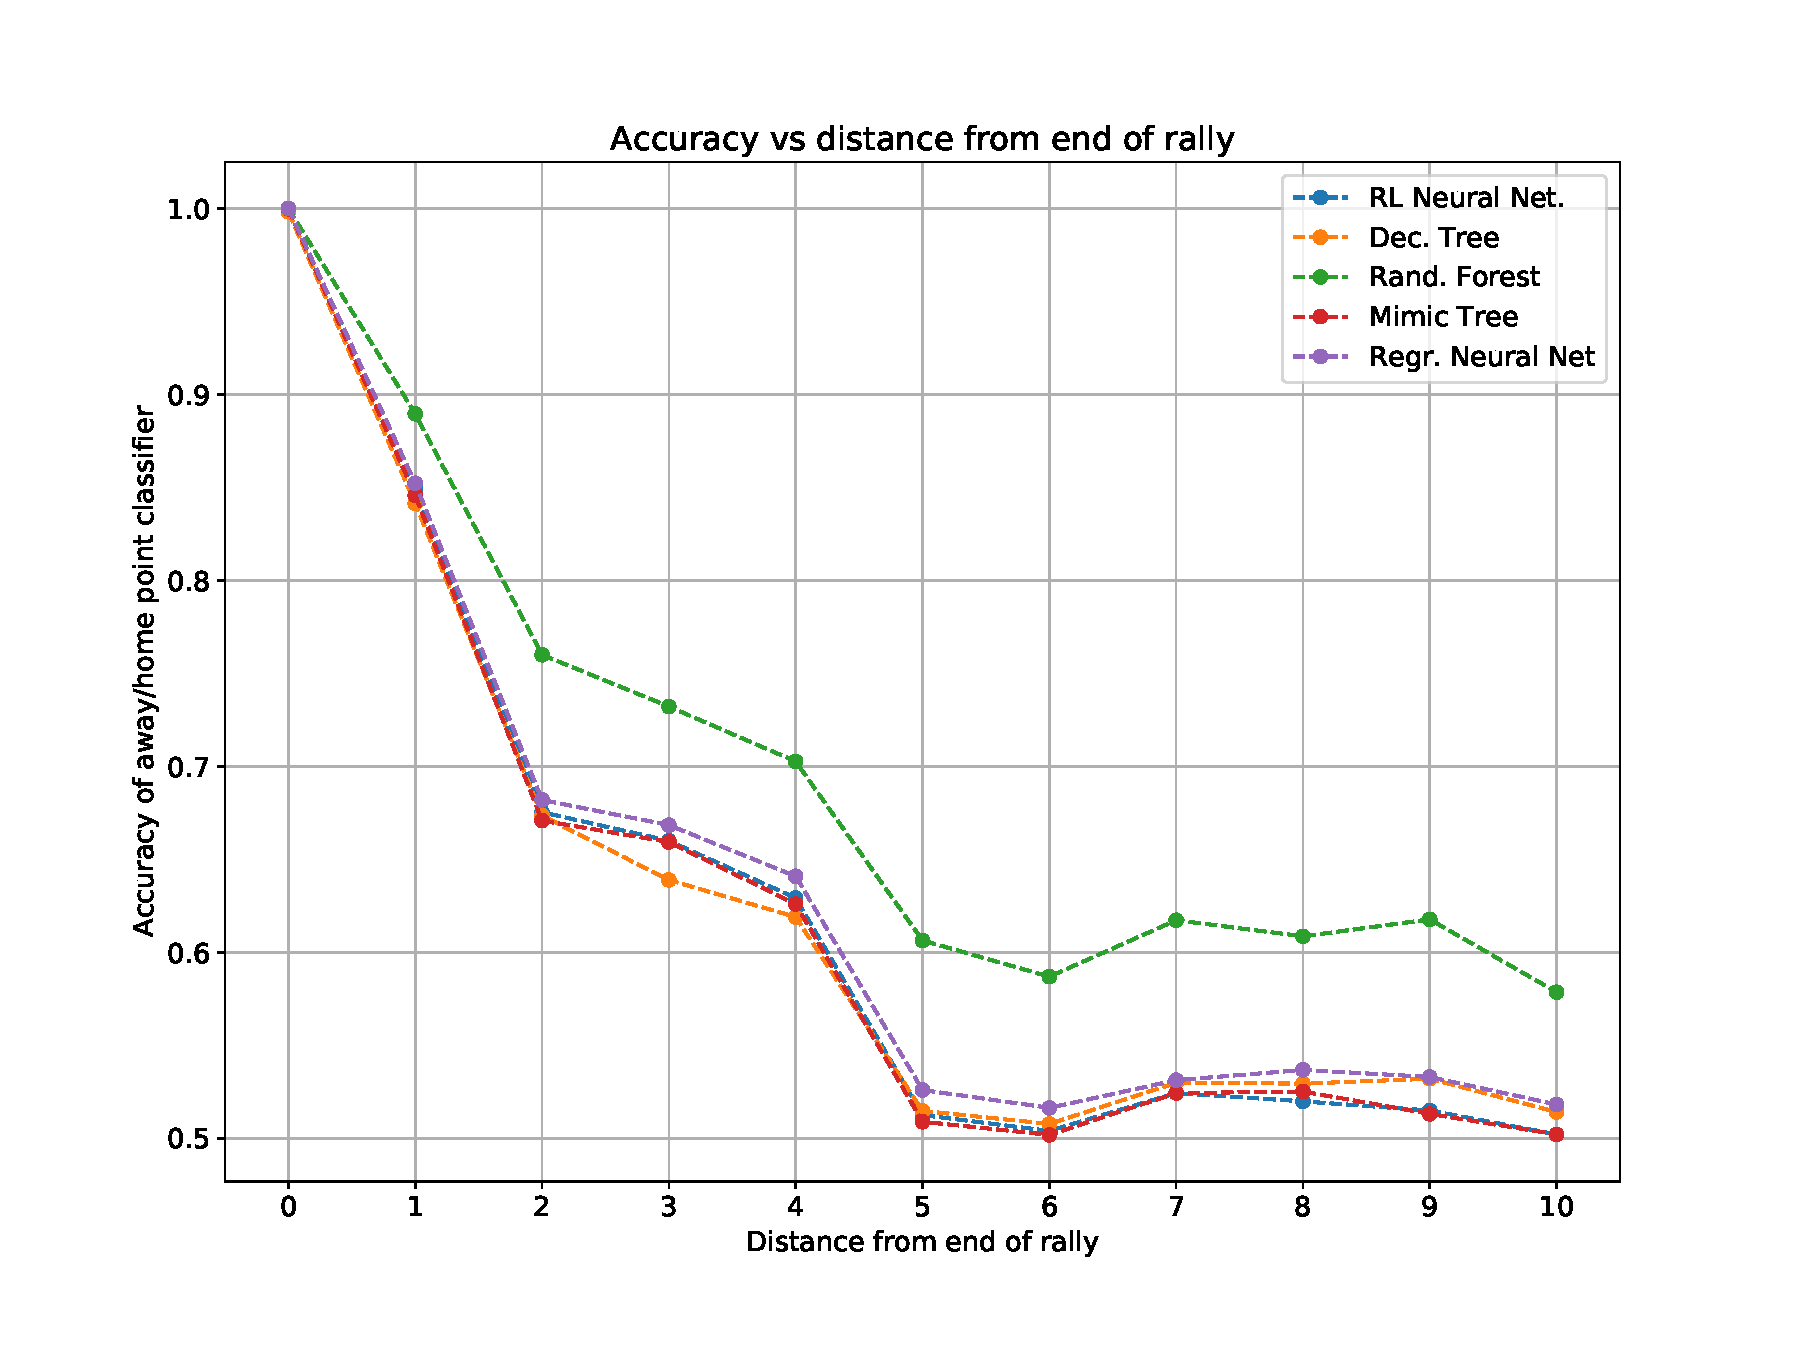
\includegraphics[scale=0.5]{img/acc_vs_dist.pdf}
		\caption{Model win prediction accuracy plotted against distance from the end of rally in terms of actions remaining.}
		\label{fig:acc-vs-dist}
	\end{figure}
	
	\chapter{Q Function Use Examples}
	
	\section{Serve Risk Assessment}
	The serve action is one of the most crucial actions types in volleyball as its outcome has a large impact on the odds of either team winning the rally. It is also the only action in volleyball where the player executing it has complete control independently of other players' actions. Optimizing the risk/reward profile for serving is therefore an important problem coaches and players frequently face \cite{burton2015linear}. In this section we examine serve action value depending on the score context, namely how close to ending the current set is in terms of score. We take $\max(\text{home score}, \text{away score})$ to be the progress measure of the current set and compare the action values of serves resulting in the '-' and '!' outcomes. The '-' outcome corresponds to the opponent team receiving the ball well enough to have all attack options available - this is the expected outcome of a serve executed with low risk. The '!' serve outcome means the opponent reception landed away from the net, removing the quick middle attack option and making opponent offence more predictable - this is generally the outcome sought when executing a serve with some (controlled) risk.
	
	Figure \ref{fig:serve-risk} shows action values converted to point scoring probability (see equation \eqref{eq:q_to_prob}) for the serve outcomes above depending on the current set score. For simplicity, the set score is bracketed into intervals of 0-5, 6-10, 11-15, 16-20 and 21-25. The x axis labels correspond to the upper end of each interval. From the graph we can observe a decreasing trend in the '-' outcome value and an increasing trend in the '!' outcome value. This would suggest a strategy using lower risk serving in the beginning of a set and gradually increasing the risk towards the end of the set, since '!' outcomes become more valuable as the set progresses.
	
	This is of course not a complete risk assessment, since we did not include any information regarding serve errors, but it can serve as an example of potential use of the action value function.
	
	\begin{figure}
		\centering
		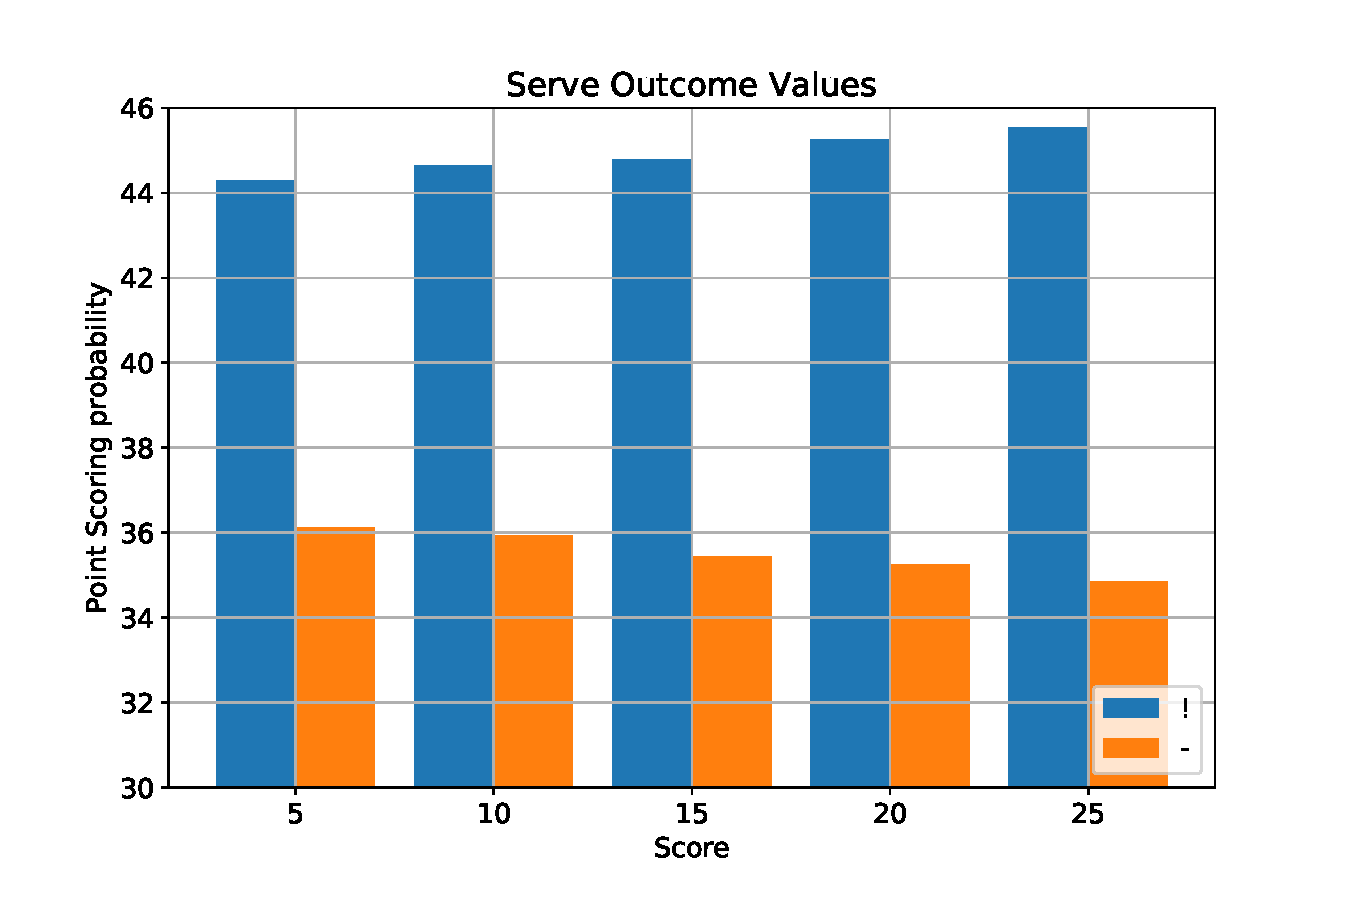
\includegraphics[scale=0.6]{img/serve_risk.pdf}
		\caption{Home serve values converted to point scoring probability for the '-' and '!' serve outcomes depending on current set score.}
		\label{fig:serve-risk}
	\end{figure}
	
	\section{Serve Receive Location Analysis}
	
	Since the previous section concerned analysis of actions through time, we now consider an example related to spatial location. We focus on the action of receiving an opponent's serve and examine the associated end location of the ball, i.e. where the ball ended up after the receive action was performed. This is a good validation example because there is ample domain knowledge on the ideal target location that we can use to compare against computed action values.
	
	Figure \ref{fig:pass-location} depicts home win probabilities by end location for the home team receiving the serve (bird's eye view of half the court is depicted with the net on the top side of the image). These can easily be computed from action values using equation \eqref{eq:q_to_prob}. Locations in the half-court furthest from the net are not included due to the fact they are not present in detail in the data.
	
	The location with highest winning probability coincides perfectly with the usual notion of a perfect reception, i.e. close to the net and shifted slightly to the right. Values generally decrease as distance from the net increases and as the location is shifted away from the ideal vertical line. This confirms our action values agree with domain knowledge and provides validation to our model.
	
	\begin{figure}[ht]
		\centering
		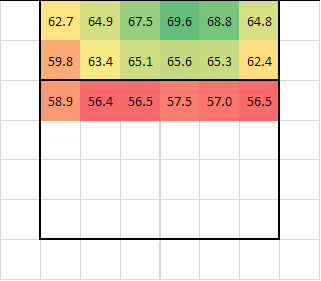
\includegraphics[scale=0.8]{img/pass_locations.png}
		\caption{Home win probabilities for serve receive actions by end location.}
		\label{fig:pass-location}
	\end{figure}
	
	\section{Action Impact}
	
	One of the motivations of computing the action-value function for sports data is the ability to numerically rank teams and players according to their action values. To achieve this, we need to consider that the context of an action performed by a player influences the quality of their actions. Namely, scoring a point from a favorable situation (eg. a successful attack following a perfect pass) should be treated differently than scoring in a situation that is deemed difficult. This leads us to the notion of action impact.
	
	As discussed in \cite{routley2015markov}, there are several options of how we could choose to value actions. We will adopt the difference of consecutive action values as a measure of impact. Namely, for a transition from state $s_{t-1}$ to $s_t$, with actions $a_{t-1}$ and $a_t$ we define the impact of $(s_t, a_t)$ as:
	\begin{equation}
		\text{impact}(s_t,a_t) = Q(s_t,a_t) - Q(s_{t-1},a_{t-1}).
		\label{eq:action_impact}
	\end{equation}
	This allows us to capture to some degree how the flow of the game changed when action $a_t$ was performed. This version of valuing player actions was successfully used in the hockey context in \cite{liu2018deep} for player evaluations.
	
	Note that since action impact relates to the values of both current and previous states, we need to find a treatment for the first action of any episode (in volleyball this is always a serve action), where $s_{t-1}$ and $a_{t-1}$ are not defined. The most obvious solution is to use an initial state-action value of 0, but since the serving team is generally at a disadvantage in terms of scoring probability, this approach gives serve actions a negative value on average and renders serve values disproportionate when compared to other action types. We therefore proceed as follows. Define $Q_{SH}$ to be the mean value of all home serve actions and $Q_{SA}$ to be the mean value of all away serve actions. We then use these values to compute action impacts as:
	\begin{equation}
		\text{impact}(s_t,a_t) =
		\begin{cases} 
			Q(s_t,a_t) - Q_{SH} & \text{if } a_t \text{ is home serve,} \\
			Q(s_t,a_t) - Q_{SA} & \text{if } a_t \text{ is away serve,} \\
			Q(s_t,a_t) - Q(s_{t-1},a_{t-1}) & \text{otherwise.} 
		\end{cases}
		\label{eq:action_impact2}
	\end{equation}
	The intuition behind this approach is to have the serve impact measure the difference between the current serve and the average serve. We also know the home team tends to have a slight advantage, which is the reason for separate averaging of home and away serves. The two means, $Q_H$ and $Q_A$ do in fact differ in absolute value by about 0.06 in favour of the home team.
	
	Firstly, we consider team collective action impact and investigate how well it aligns with team performance in the Canada West volleyball competition in the last three seasons. To this end, we compute the mean impact of all actions performed by players of a particular team using equation \eqref{eq:action_impact2}. These values are collected in Table \ref{tab:team-impact} for all teams participating in the Canada West men's volleyball competition (with the exception of Regina, who ceased participation after the 2017/2018 season and is not well represented in the dataset). We compare action impact values to mean ranking of the teams following regular season across the 2017/2018, 2018/2019 and 2019/2020 seasons, also included in Table \ref{tab:team-impact}. Teams in the table are sorted by mean action impact. Good alignment against team ranking can be seen from inspection of the table, but a plot is also included in Figure \ref{fig:team-impact} for a more visual representation. With the exception of three teams, an increase in mean action impact corresponds to higher ranking, which is desirable behaviour for our model, as higher action values lead to more wins. We also compute the Pearson correlation coefficient between mean action impacts and mean rankings and obtain a value of -0.854, confirming a high correlation and a near linear relationship.
	\begin{table}[ht]
		\centering
		\begin{tabular}{cccccc}
			\textbf{Team}   & \textbf{Mean Action Impact} & \textbf{R20} & \textbf{R19} & \textbf{R18} & \textbf{Mean Ranking} \\ \hline
			Trinity Western & 0.0220                      & 1            & 2            & 1            & 1.33                  \\
			Alberta         & 0.0175                      & 2            & 3            & 3            & 2.67                  \\
			UBC             & 0.0124                      & 3            & 7            & 2            & 4.00                  \\
			Brandon         & 0.0077                      & 4            & 1            & 4            & 3.00                  \\
			Calgary         & 0.0073                      & 5            & 8            & 6            & 6.33                  \\
			Winnipeg        & 0.0053                      & 6            & 10           & 5            & 7.00                  \\
			Mount Royal     & -0.0053                     & 8            & 4            & 10           & 7.33                  \\
			Manitoba        & -0.0067                     & 10           & 9            & 7            & 8.67                  \\
			MacEwan         & -0.0128                     & 12           & 11           & 12           & 11.67                 \\
			Thompson Rivers & -0.0144                     & 9            & 6            & 8            & 7.67                  \\
			Saskatchewan    & -0.0210                     & 7            & 5            & 9            & 7.00                  \\
			UBCO            & -0.0235                     & 11           & 12           & 11           & 11.33                
		\end{tabular}
		\caption{Canada West teams sorted by mean action impact. Columns R20, R19, R18 are team rankings after regular season in 2020, 2019 and 2018, respectively and Mean Ranking is the mean of those three columns.}
		\label{tab:team-impact}
	\end{table}
	
	We note here again that the dataset contains all UBC games, but not all games among other Canada West teams, meaning that the amount of data for those teams is significantly lower than for UBC. The bias introduced by this could explain the outliers in Figure \ref{fig:team-impact}.
	
	We can compute mean action impacts for individual players in the same fashion as we did for teams above, which enables us to track and rank player performance. Table \ref{tab:player-impact} shows the top 10 players ranked by mean action impact in Canada West. The caveat, compared to team ranking, is that there are fewer obvious ways to check the validity of these values. In professional leagues such as the NHL, player salary has been used for this purpose, e.g. in \cite{schulte2017apples}, but there is no such information for university athletes. Regardless, we still attempt some discussion. Notably, most of the players listed come from the top ranked teams - the best 4 teams in Canada West (by mean ranking in the last 3 seasons) are represented 8 out of 10 times, which can be taken as a good sign.
	
	On a more individual level, player awards and recognition can provide further validity to our ranking. Elliot Viles, who ranks first in Table \ref{tab:player-impact}, was named a conference all-star in his rookie season and both Canada West as well as U SPORTS National player of the year in the 2018/2019 season. He also represented his home country Australia in the prestigious FIVB World League competition. Eric Loeppky, who follows closely in the mean impact ranking, also received the title of U SPORTS player of the year in 2020 as well as multiple other awards and has played on the Canadian senior national team, which is rare for players still in their university years. Jackson Kennedy and Daniel Thiessen have furthermore been selected as Canada West all-star team members alongside Loeppky and Viles. Prominent players like that featuring as leaders in impact ranking is further validation of our action impact model.
	\begin{table}
		\centering
		\begin{tabular}{ccc}
			\textbf{Player Name} & \textbf{Team}   & \textbf{Mean Action Impact} \\ \hline
			Elliot Viles         & Brandon         & 0.0838                      \\
			Eric Loeppky         & Trinity Western & 0.0796                      \\
			Jackson Kennedy      & Alberta         & 0.0580                      \\
			George Hobern        & Alberta         & 0.0566                      \\
			Hamish Hazelden      & Calgary         & 0.0539                      \\
			Joel Regher          & UBC             & 0.0509                      \\
			Daniel Thiessen      & Winnipeg        & 0.0504                      \\
			Gerard Murray        & UBC             & 0.0471                      \\
			Jordan Canham        & Alberta         & 0.0459                      \\
			Arran Chambers       & Alberta         & 0.0451                     
		\end{tabular}
		\caption{Top 10 individual players in Canada West by mean action impact as given in equation \eqref{eq:action_impact2}.}
		\label{tab:player-impact}
	\end{table}
	
	\begin{figure}
		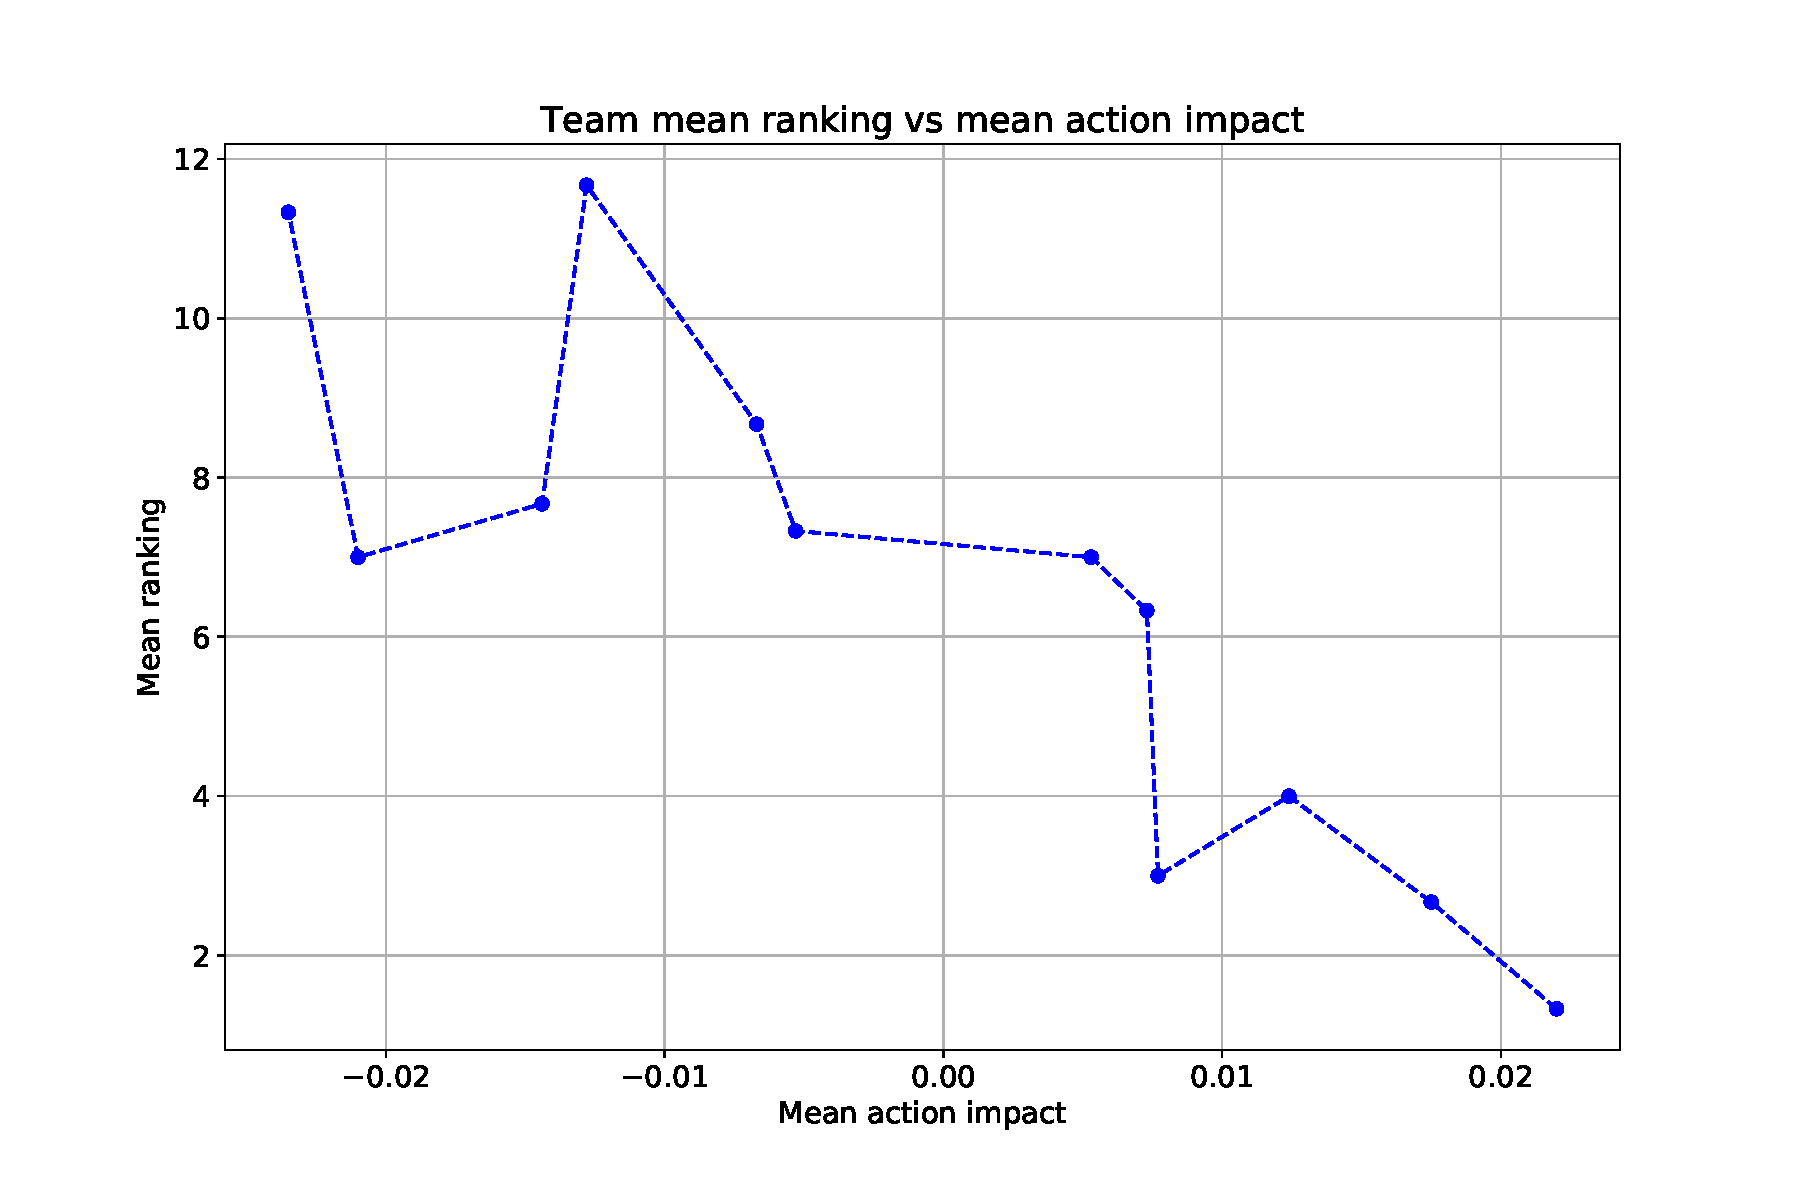
\includegraphics[scale=0.55]{img/team_ranking.pdf}
		\caption{Team mean ranking plotted against mean action impact for Canada West participating teams, see Table \ref{tab:team-impact} for values shown in this graph.}
		\label{fig:team-impact}
	\end{figure}
	
	\chapter{Conclusion and Future Work}
	
	This project explores learning action values from volleyball data using two fundamentally different approaches. In the first approach, regression models are used to estimate the eventual reward (winning the rally) using partial action sequences and match context under an independence assumption. In the second approach, deep reinforcement learning is used, explicitly incorporating the sequential nature of the data into the learning process.
	
	In terms of mean squared error, a common measure used in regression, the random forest regression model achieved the best fit out of all experiments, followed by the RL neural network in second place. However, when considering temporal consistency, the reinforcement learning approach produced much more consistent action values. This suggests that the random forest might be of better use in a strictly predictive context, but since action values can be used in a diverse range of sports analyses (a sample of which we include in Chapter 5), we believe the temporal consistency of deep reinforcement learning makes it the best choice.
	
	As an additional experiment, we include a tree regression model based on mimic learning. We find that it can achieve good fidelity to the RL neural network's outputs (see Table \ref{tab:mimic-mse}), while providing insight into their interpretation through its tree structure.
	
	In Chapter 5, a number of example analyses using action values are carried out using the values computed by the RL neural network. Comparing those against domain knowledge we find a high degree of agreement, which adds validity to our model.
	
	In terms of future work, this project examines only a small subset of all available machine learning models, so there are numerous possible extensions:
	\begin{itemize}
		\item Additional ensemble methods for regression could be tested, e.g. gradient boosted trees.
		\item When performing mimic learning, we restrict ourselves to a regression tree, but a linear model tree could be used such as in \cite{sun2020cracking}.
		\item Finally, there are numerous architecture choices in neural network design that could be considered, such as convolutional neural networks.
	\end{itemize}  
	
	%   BACK MATTER  %%%%%%%%%%%%%%%%%%%%%%%%%%%%%%%%%%%%%%%%%%%%%%%%%%%%%%%%%%%%%%
	%
	%   References and appendices. Appendices come after the bibliography and
	%   should be in the order that they are referred to in the text.
	%
	%   If you include figures, etc. in an appendix, be sure to use
	%
	%       \caption[]{...}
	%
	%   to make sure they are not listed in the List of Figures.
	%
	
	\backmatter%
	\addtoToC{Bibliography}
	\bibliographystyle{plain}
	\bibliography{msc_report}
	
	\begin{appendices} % optional
		\chapter{Code}
	\end{appendices}
\end{document}
